\documentclass{report}
\usepackage{graphicx}
\newcommand{\T}[1]{$\Theta$(#1)}
\title{
    Introduzione agli algoritmi \\
}

\begin{document}
\maketitle
\tableofcontents

\newpage
\detokenize{https://mega.nz/folder/4osyiZAI#2I2lpukRbJ-n7-HsmHLxhA/folder/x1szTAhI}
\section{RAM}
    La RAM è la componente del computer che si occupa di memorizzare i bits.
    I byte, struttura minima indirizzabile, con l'indirizzo che corrisponde
    allo scostamento in bytes dall'inizio del memory block del programma, dalla CPU, 
    sono raggruppati a loro volta in \textbf{words}, l'unità massima quali la 
    CPU può operare con una \textbf{singola} istruzione. \\
    Il tempo impiegato dalla RAM per accedere a un byte è \T{1}. \\
    Il numero massimo di indirizzi usabili è detto \textbf{spazio di memorizzazione}, 
    e corrisponde alla lunghezza di una word nel sistema preso in considerazione.
\section{Il modello random access machine}
    Il modello usato nell'analisi della complessità computazionale di un algoritmo. \\
    Le caratteristiche sono:
    \begin{itemize}
        \item possiede un singolo processore che effettua operazioni sequenzialmente
        \item possiede un insieme di \textbf{operazioni elementari} dal costo \T{1}
        \item possiede un \textbf{limite} massimo di grandezza per ogni valore memorizzato
            e per lo spazio di indirizzamento
    \end{itemize}
\section{Criterio di misurazione del costo}
    \subsection{Criterio di misurazione del costo uniforme}
        Data la dimensione \textit{d} di una word, se tutti i dati hanno grandezza $ < $ \textit{d}, 
        le operazioni elementari su essi avranno costo \T{1}. \\
        Non molto realistico in quanto molto spesso i dati hanno grandezza $ > $ \textit{d}
        ma spesso usato in quanto più semplice
    \subsection{Criterio di misurazione del costo logaritmico}
        Criterio più realistico ma che rende le misurazioni più complicate, afferma 
        che il costo di una singola operazione su un dato di grandezza n è $\log_{2}n$. 
\section{Notazione asintotica}
    La notazione asintotica è un modello astratto che descrive, in termini di 
    tempo d'esecuzione e/o di memoria usata, il \textbf{tasso di crescita} del
    costo di una funzione in base alla grandezza dell'input.
    \subsection{Notazione O}
        Prese $f\left(n\right), \, g\left(n\right) \geq 0$ si dice che $f(n)$ è un O(g(n)) se 
        $$\exists c, \, n_0 \textrm{ t.c. } c*g\left(n\right) \geq f\left(n\right) \geq 0 \, \forall n \geq n_0$$
        Di infinite funzioni $g\left(n\right)$ a noi interessa quella che meglio approssima $f\left(n\right)$ 
        dall'alto
    \subsection{Notazione $\Omega$}
        Come la notazione O, solo che approssimiamo dal basso.
    \subsection{Notazione $\Theta$}
        f(n) è un \T{g(n)} quando f(n) è O(g(n)) $\wedge \Omega$g(n)
    \subsection{Algebra della notazione asintotica}
        $$\forall k > 0, \, f\left(n\right) \geq 0, \, f\left(n\right) \textrm{ è un }
            O/\Omega/\Theta\left(g\left(n\right)\right) \Longrightarrow k * f\left(n\right) \textrm{ è un }
            O/\Omega/\Theta\left(g\left(n\right)\right)$$

        $$\forall f\left(n\right), \, d\left(n\right) \geq 0, f\left(n\right) \textrm{ è un }
            O/\Omega/\Theta\left(g\left(n\right)\right) \, \wedge \, d\left(n\right) \textrm{ è un }
            O/\Omega/\Theta\left(h\left(n\right)\right) \Longrightarrow$$
        $$f\left(n\right) + d\left(n\right) \textrm{ è un } 
            O/\Omega/\Theta\left(\textrm{max}\left(g\left(n\right), h\left(n\right)\right)\right)$$

        $$\forall f\left(n\right), \, d\left(n\right) \geq 0, f\left(n\right) \textrm{ è un }
            O/\Omega/\Theta\left(g\left(n\right)\right) \, \wedge \, d\left(n\right) \textrm{ è un }
            O/\Omega/\Theta\left(h\left(n\right)\right) \Longrightarrow$$
        $$f\left(n\right) * d\left(n\right) \textrm{ è un } 
            O/\Omega/\Theta\left(g\left(n\right) * h\left(n\right)\right)$$
    \subsection{Calcolo della notazione asintotica tramite limiti}
        $\lim_{n \to \infty}\frac{f\left(n\right)}{g\left(n\right)} =$
        \begin{itemize}
            \item $k > 0 \Longrightarrow f\left(n\right) = $ \T{g(n)}
            \item $\infty \Longrightarrow f\left(n\right) = \Omega\left(g\left(n\right)\right)
                \neq$ \T{$g\left(n\right)$}
            \item $0 \Longrightarrow f\left(n\right) = O\left(g\left(n\right)\right)
                \neq$ \T{$g\left(n\right)$}
        \end{itemize}
\section{Ccosto computazionale di un algoritmo}
    \subsection{Calcolo del costo}
    \begin{enumerate}
        \item Individuare la \textbf{dimensione dell'input}
        \item Formulare in modo chiaro l'algoritmo in \textbf{pseudocodice}
        \item Seguire le regole base:
            \begin{itemize}
                \item le operazioni elementari hanno costo \T{1}
                \item l'istruzione \verb|if cond then st1 else st2| ha come costo
                    la somma fra il costo di verifica della condizione e il massimo dei
                    costi di st1 ed st2
                \item l'istruzioni iterative hanno come costo la somma fra la verifica 
                    della condizione * n e la somma dei costi massimi di ogni singola 
                    interazione (spesso uguale)
                \item Il costo dell'algoritmo è la somma dei costi di tutte le istruzioni
            \end{itemize}
        \item Quando un algoritmo potrebbe avere costi diversi in base all'input, occorre
            valutare anche il \textbf{caso migliore} ed il \textbf{caso peggiore}
        \item Quando si valuta il costo di un algoritmo senza conoscere l'input
            bisogna sempre considerare il caso peggiore
    \end{enumerate}
    \subsection{I problemi intrattabili e l'importanza dell'efficienza}
        Si chiamano problemi intrattabili quei problemi che, data una dimensione 
        realistica dell'input, il costo computazionale è proibitivo. \\
        Per questo, quando si progetta un algoritmo oltre alla correttezza dello
        stesso è fondamentale risolverlo in modo efficiente
\newpage
\section{Problema della ricerca}
    Problema molto ricorrente, si analizza nella versione con I = A[] ed output 
    l'indice dell'elemento x cercato in A[].
    \subsection{Soluzione sequenziale}
    \begin{itemize}
        \item Semplice
        \item Caso peggiore: \T{n}
        \item Caso migliore: \T{1}
        \item Analisi del costo: considerando ogni possibile posizione di x
            come equiprobabile, il numero medio di iterazione è 
            $$\Sigma_{i=1}^{n} i\frac{1}{n} = \frac{1}{n}*\frac{n*\left(n+1\right)}{2} = \textrm{\T{n}}$$
    \end{itemize}
    \subsection{Ricerca binaria}
    \begin{itemize}
        \item Prerequisito: A[] è ordinato
        \item Caso peggiore: \T{$\log_2n$}
        \item Caso migliore: \T{1}
        \item Analisi del costo: ad ogni iterazione i escludiamo $2^{i-1}-1$ posizioni
            e ne confrontiamo 1. Quindi, il numero medio di iterazioni è
            $$\Sigma_{i=1}^{\log_2n}i\frac{2^{i-1}-1 + 1}{n} = 
                \frac{1}{n}\Sigma_{i=1}^{\log_2n}i2^{i-1} = $$
            $$\frac{1}{n}\left(\left(\log_2n - 1\right)2^{\log_2n}+1\right) = 
                \log_2n - 1 + \frac{1}{n}$$
    \end{itemize}
\section{Ricorsione}
    Un algoritmo \textbf{ricorsivo} è espresso in termini di se stesso. \\
    La successione dei sottoproblemi che dividono la soluzione deve convergere 
    verso uno o più \textbf{casi base} che termina la ricorsione. \\
    Di norma, una soluzione ricorsiva ha \textbf{costi maggiori}, in termini di memoria e 
    tempo di esecuzione, rispetto a una soluzione iterativa, dati dai costi intrinsechi
    dell'uso delle funzioni. \\
    Una soluzione ricorsiva può sempre essere espressa anche come soluzione iterativa. \\
    La ricorsione è detta \textbf{diretta} se $f$ chiama $f$, mentre è \textbf{indiretta} se $f$ chiama $g$ che
    chiama $f$
    \subsection{Calcolare il costo di una funzione ricorsiva}
        La prima cosa da fare è impostare l'\textbf{equazione di ricorrenza}, costituita dalla formulazione
        ricorsiva e dal caso base. \\
        Ad esempio, poniamo di avere un algoritmo che fa un test su $x \in A\left[\right]$ che, 
        se soddisfatto interrompe la ricorsione, in caso contrario effettua una chiamata ricorsiva 
        su $A\left[1:\right]$. Il costo computazionale dell'algoritmo A è quindi: 
        \begin{itemize}
            \item T(n): T(n-1) + \T{n}
            \item T(1): \T{n}
        \end{itemize}
        \subsubsection{Metodo di sostituzione}
        \begin{enumerate}
            \item si ipotizza una soluzione per l'equazione di ricorrenza
            \item per \textbf{induzione}, si verifica la correttezza della soluzione
        \end{enumerate}
            La vera difficoltà nel metodo sta nel trovare $O$ ed $\Omega$ che meglio
            approssimano $f$. \\
            Prendendo l'algoritmo A, proviamo a calcolarne il costo col metodo di sostituzione. \\
        \begin{enumerate}
            \item Sostituiamo le notazioni asintotiche con costanti:
            \begin{itemize}
                \item T(n) = T(n-1) + c (c $> 0$)
                \item T(1) = d (d $> 0$)
            \end{itemize}
            \item Ipotizziamo T(n) = O(n), con T(n) $\leq k*n$ con $k$ da determinare
            \item Nel caso base abbiamo quindi T(1) $\leq k*n = k * 1 \Longrightarrow d \leq k$
            \item Assumiamo quindi T(r) $\leq k*r \forall r < n \Longrightarrow$
            \item T(n) = T(n-1) + c $\leq kn \Longrightarrow$ T(n) $\leq k(n-1) + c \leq kn \Longrightarrow k \geq c$
            \item L'ipotesi è quindi vera $\forall k \geq c, \, d \Longrightarrow$ T(n) è un O(n)
            \item Ipotizziamo ora T(n) = $\Omega$(n), con T(n) $\geq hn$ con $h$ da determinare
            \item Analogamente a prima, T(1) $\geq hn = h \Longrightarrow d \geq h$
            \item Sempre analogamente a prima assumiamo T(r) $\geq hr \forall r < n \Longrightarrow$
            \item T(n) = T(n-1) + c $\geq hn \Longrightarrow$ T(n) $\geq h(n-1) + c \geq hn \Longrightarrow h \leq c$
            \item L'ipotesi è quindi vera $\forall h \leq c, \, d \Longrightarrow$ T(n) è un $\Omega$(n)
            \item Essendo T(n) un $\Omega$(n) ed un O(n) $\Longrightarrow$ T(n) è un \T{n}
        \end{enumerate}
            Analizziamo ora un altro caso definito da:
            \begin{itemize}
                \item T(n) = 2T($\frac{n}{2}$) + \T{1}
                \item T(1) = \T{1}
            \end{itemize}
            \begin{enumerate}
                \item Sostituiamo le notazione asintotiche con costanti:
                \begin{itemize}
                    \item T(n) = 2T{$\frac{n}{2}$} + c (c $>$ 0)
                    \item T(1) = d (d $>$ 0)
                \end{itemize}
                \item Ipotizziamo T(n) = O(n), con T(n) $\leq kn$ 
                \item Nel caso base abbiamo quindi T(1) $\leq kn = k \Longrightarrow d \leq k$
                \item Analogamente a prima, T(n) = 2T($\frac{n}{2}$) + c $\leq kn \Longrightarrow$
                    T(n) $\leq$ 2*($k*\frac{n}{2}$) + c $\leq kn \Longrightarrow$ \\
                    T(n) $\leq kn + c \leq kn \Longrightarrow c \leq 0$, impossibile in quanto
                    c è per definizione $>$ 0. 
                \item La funzione quindi non è limitata superiormente da $kn$
                \item Proviamo con T(n) $\leq kn - h$
                \item Caso base: T(1) $\leq kn - h = k - h \Longrightarrow d + h \leq k$
                \item T(n) = 2($k*\frac{n}{2} - h) + c \leq kn - h \Longrightarrow kn - 2h + c \leq kn - h 
                    \Longrightarrow$ \\ $c - h \leq 0 \Longrightarrow c \leq h \Longrightarrow$
                \item T(n) è un O(n)
                \item Analogamente possiamo dimostrare che T(n) è un $\Omega$(n)
            \end{enumerate}
        \subsubsection{Metodo iterativo}
            L'idea di base è di sviluppare l'equazione di ricorrenza come \textbf{somma fra caso base e termini dipendenti da n}. \\
            Prendendo la funzione di prima:
            \begin{enumerate}
                \item T(n) = T(n-1) + \T{1}, T(n-1) = T(n-2) + \T{1} $\Longrightarrow$
                \item T(n) = T(n-2) + \T{1} + \T{1}, T(n-2) = ... $\Longrightarrow$
                \item T(n) = T(1) + (n-1)\T{1}, T(1) = \T{1} $\Longrightarrow$
                \item T(n) = n\T{1} = \T{n}
            \end{enumerate}
            Non tutte le equazione di ricorrenza sono però efficacemente risolvibili col metodo classico, per esempio 
            l'algoritmo della sequenza di fibonacci:
            \begin{itemize}
                \item T(n) = T(n-1) + T(n-2) + \T{1}
                \item T(0) = T(1) = \T{1}
            \end{itemize}
            \begin{enumerate}
                \item Possiamo però notare che 2T(n-2)+\T{1} $\leq$ T(n) $\leq$ 2T(n-1) + \T{1}
                \item Risolviamo il limite superiore: \\
                    T(n) $\leq$ 2T(n-1) + \T{1} $\leq 2^2$T(n-2) + 3\T{1} $leq 2^3$T(n-3) + 7\T{1} $\Longrightarrow$ \\
                    $\leq 2^k$T(n-k) + $\left(2^k-1\right)$\T{1}, che si ferma con $k=n-1$, per cui otteniamo: \\
                    T(n) $\leq 2^{n-1}$\T{1} $+ \left(2^{n-1}-1\right)$\T{1} $ = \left(2^n-1\right)$\T{1} $\Longrightarrow$
                \item T(n) è un O($2^n$)
                \item Analogamente risolviamo il limite inferiore: \\
                    T(n) $\geq$ 2T(n-2) + \T{1} $\geq 2^2T(n-4) + 3$\T{1} $\Longrightarrow$ \\
                    $\geq 2^k$T(n-2k) + $\left(2^k-1\right)$\T{1}, che si ferma con $k=\frac{n}{2}$ per cui otteniamo: \\
                    T(n) $\geq 2^{\frac{n}{2}}$\T{1} + $\left(2^{\frac{n}{2}}-1\right)$\T{1} $ = \left(2^{\frac{n+1}{2}}-1\right)$\T{1} $\Longrightarrow$
                    T(n) è un $\Omega\left(2^{\frac{n}{2}}\right)$
                \item Quindi, $k_12^{\frac{n}{2}} \leq$ T(n) $\leq k_22^n$
            \end{enumerate}
            \subsubsection{Metodo dell'albero}
                La costruzione dell'\textbf{albero di ricorrenza} è un metodo 
                grafico per la rappresentazione del costo computazionale. \\
                Ogni nodo è relativo alla soluzione dei problemi per una certa dimensione
                k, ed ha tznti figli quante sono le chiamate ricorsive il cui il nodo stesso 
                è scomposto. \\
                Riporta il \textbf{costo della ricombinazione delle soluzioni parziali}. \\
                Per esempio, l'albero dell'equazione di ricorrenza:
                \begin{itemize}
                    \item T(n) = 2T(n/2) + \T{n$^2$}
                    \item T(1) = \T{1}
                \end{itemize}
                è:
                \begin{center}
                    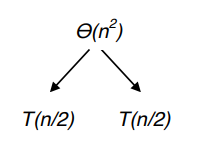
\includegraphics{albero.png}
                \end{center}
                Si applica poi ricorsivamente il processo su ognuno dei figli.
            \subsubsection{Metodo del teorema principale}
                Fornisce una risoluzione meccanica per le equazioni nella forma:
                \begin{itemize}
                    \item T(n) = aT(n/b) + f(n) (a $\geq$ 1, b $>$ 1 e f(n) asintoticamente positiva)
                    \item T(1) = \T{1}
                \end{itemize}
                Il teorema enuncia che, rispettate le ipotesi espresse sopra, se $f\left(n\right)$:
                \begin{itemize}
                    \item $= O\left(n^{\log_ba-\epsilon}\right)$ per $\epsilon > 0 
                        \Longrightarrow T\left(n\right) = $\T{$n^{\log_ba}$}
                    \item $= $ \T{$n^{\log_ba}$} $
                        \Longrightarrow T\left(n\right) = $ \T{$n^{\log_ba}\log_2n$}
                    \item $= \Omega\left(n^{\log_ba+\epsilon}\right)$ per $\epsilon > 0$ e 
                        se $af\left(n/b\right) < cf\left(n\right)$ per $c < 1$ ed $n$ sufficientemente
                        grande $\Longrightarrow T\left(n\right)$ = \T{$f\left(n\right)$}
                \end{itemize}
                In termini più semplici, enuncia che se $f\left(n\right)$:
                \begin{itemize}
                    \item $> n^{\log_ba}$ allora $T\left(n\right)$ = \T{$f\left(n\right)$}
                    \item $= n^{\log_ba}$ allora $T\left(n\right)$ = \T{$n^{\log_ba}\log_2n$}
                    \item $< n^{\log_ba}$ allora $T\left(n\right)$ = \T{$n^{\log_ba}$}
                    \item A patto che $|f\left(n\right) - n^{\log_ba}| > n^\epsilon, \, \epsilon > 0$   
                \end{itemize}
                Alcuni esempi:
                \begin{enumerate}
                    \item \begin{itemize}
                        \item T(n) = 9T(n/3) + \T{n}
                        \item T(1) = \T{1}
                        \item a = 9, b = 3, f(n) = \T{n}
                        \item $n^{\log_ba} = n^{\log_39} = n^2$
                        \item $n < n^2 \Longrightarrow T\left(n\right) =$ \T{$n^2$}
                    \end{itemize}
                    \item \begin{itemize}
                        \item T(n) = T(2n/3) + \T{1}
                        \item T(1) = \T{1}
                        \item a = 1, b = 3/2, f(n) = \T{1}
                        \item $n^{\log_ba} = n^{log_{3/2}1} = n^0 = 1$
                        \item $1 = 1 \Longrightarrow T\left(n\right)$ = \T{$1 * log_2n$}
                    \end{itemize}
                    \item \begin{itemize}
                        \item T(n) = 3T(n/4) + \T{$n\log_2n$}
                        \item T(1) = \T{1}
                        \item a = 3, b = 4, f(n) = \T{$n\log_2n$}
                        \item $n^{\log_43} = n^{0<x<1}$
                        \item $n\log_2n > n^{0<x<1}$
                        \item $\frac{3n}{4}\log_2\frac{n}{4} \leq c(n\log_2n), \, c < 1 
                            \Longrightarrow \frac{3n}{4}\log_2\frac{n}{4} \leq \frac{3}{4}(n\log_2n)
                            \Longrightarrow$
                        \item $T\left(n\right)$ = \T{$n\log_2n}$
                    \end{itemize}
                \end{enumerate}
\section{Esercizi}
    \detokenize{https://mega.nz/folder/4osyiZAI#2I2lpukRbJ-n7-HsmHLxhA/folder/l1tXEIrS}
    \subsection{1}
        Il caso peggiore è \T{n} in quanto scorre tutti i numeri da 1 ad n per poi effettuare 
        un'operazione \T{1}. \\
        Esiste una versione \T{1} per effettuare il calcolo col metodo di Gauss: $\frac{n\left(n\right)}{2}$
    \subsection{2}
        
        

\end{document}
        
    